\chapter{Wprowadzenie}
\label{cha:wprowadzenie}

W~tym rozdziale przedstawiono cel pracy oraz podstawę teoretyczną realizacji. Opisano szczegółowo implementowany algorytm Scale Space: podstawy matematyczne i~sposób działania. Przybliżono również standard OpenCL, który został wykorzystany do realizacji algorytmu.


\section{Cel pracy}
\label{sec:cel}
Celem niniejszej pracy była realizacja algorytmu Scale Space, który służy do reprezentacji sygnałów (w~szczególności obrazów) w~wielu skalach w celu późniejszej ich analizy.
Wiele algorytmów operujących na obrazach jest złożonych obliczeniowo i~ich realizacja zajmuje dużo czasu, zwłaszcza dla dużych porcji danych. Dlatego zdecydowano się na realizację tego algorytmu w~postaci równoległej z~użyciem kart graficznych.

Implementacja algorytmu została zrealizowana w~środowisku OpenCL \cite{OpenCL}, wieloplatformowym standardzie do zrównoleglania obliczeń. Wybrano ten standard, ponieważ umożliwia wykorzystanie procesorów graficznych do obliczeń ogólnego przeznaczenia oraz jest wspierany przez największych producentów sprzętu komputerowego (m. in. Intel\textsuperscript{\textregistered}, NVIDIA\textsuperscript{\texttrademark}, AMD).

\section{Algorytm Scale Space}
\label{sec:algorytm}
Scale Space jest algorytmem służącym do przekształcenia sygnałów do reprezentacji skali \cite{SSFramework}. Reprezentacja skali jest to rodzina sygnałów reprezentująca oryginalny sygnał w~różnych stopniach skali.
Ta reprezentacja pozwala na analizę oryginalnego sygnału w~różnych stopniach szczegółowości.
Pomysł na stworzenie takiego algorytmu wynika z~wieloskalowej struktury świata. Taka struktura powoduje, że obiekty mogą być różnie postrzegane w~zależności od skali obserwacji \cite{Enc09}.
W~tej pracy przetwarzanymi sygnałami będą obrazy.

Tworząc system automatycznego rozpoznawania obrazów nieznanych scen nie ma możliwości określenie z~góry w~jakiej skali będą przedstawiane obiekty, które będą interesujące dla użytkownika systemu. Dlatego w~takim systemie można użyć algorytmu Scale Space wraz z~automatycznym rozpoznawaniem najbardziej interesującej skali. Po stworzeniu reprezentacji skali można zrealizować rozpoznawanie plam, narożników, grani lub brzegów. Te operacje mogą być przeprowadzane tylko w~jednej skali lub dla większej liczby skal, w~szczególności we wszystkich skalach.

\subsection{Aksjomaty Scale Space}
\label{subsec:aksjomaty}

Operator wykorzystywany do wyznaczenia reprezentacji skali musi spełniać przedstawione poniżej warunki nazwane aksjomatami Scale Space. 

\begin{enumerate}
\item Nie tworzenie nowych lokalny ekstremów.

Pierwszą istotną kwestią jest to, by podczas uzyskiwania wartości sygnałów dla większych skali nie były tworzone nowe lokalne ekstrema. Celem uzyskiwania sygnału w~większej skali jest ograniczenie liczby szczegółów widocznych w~sygnale w~skali mniejszej. Dlatego liczba lokalnych ekstremów powinna być mniejsza lub równa przy zwiększaniu skali.

\item Nie zwiększanie wartości lokalnych ekstremów

Kolejnym ważnym elementem przy wyznaczaniu reprezentacji skali jest nie zwiększanie wartości lokalnych ekstremów. Przez nie zwiększanie wartości jest rozumiane to, że maksimum lokalne w~większej skali będzie miało wartość mniejszą lub równą wartości w~skali mniejszej, natomiast minimum lokalne wraz ze wzrostem skali powinno mieć wartość większą lub równą.

\end{enumerate}

Sygnał w reprezentacji skali może być w przestrzeni ciągłej lub dyskretnej. Dodatkowo parametr skali może być ciągły lub dyskretny. W tej pracy przetwarzane będą sygnały dyskretne (obrazy) przy użyciu dyskretnym parametrze skali.

Dla sygnałów dyskretnych przy użyciu dyskretnego parametru skali należy przyjąć pewne założenia~\cite{SSFDS}:
\begin{itemize}
\item Cała reprezentacja skali jest stworzona z~obrazu źródłowego za pomocą jednej rodziny filtrów.
\item Wraz ze zwiększaniem parametru skali $ t $ otrzymywane sygnały odpowiadają większym skalom. Przy $ t = 0 $ otrzymanym obrazem jest obraz źródłowy.
\item Wszystkie sygnały są funkcjami: $ Z -> R $ zdefiniowane na tym samym skończonym zbiorze.
\end{itemize}

Istotne jest to, aby sygnały dla większych skal zawierały mniej szczegółów. Liczba szczegółów może być określona za pomocą ilości lokalnych ekstremów. Dlatego istotne jest to, aby liczba lokalnych ekstremów nie zwiększała się wraz ze wzrostem parametru skali.

\subsection{Filtracja Gaussa}
\label{subsec:filtracjaGaussa}
Filtry Gaussa są jednymi z podstawowych operacji wykorzystywanych w przetwarzaniu obrazów cyfrowych. Są to filtry dolnoprzepustowe, rozmywające obraz, po zastosowaniu których ze sceny można odczytać ogólne kształty przedstawionych obiektów. Po tej operacji szczegóły zostają usunięte, bądź zostaje znacznie zmniejszony ich wpływ na całość. Ich zaletą wykorzystywaną w~tej pracy jest ich zgodność z aksjomatami Scale Space zarówno w~postaci ciągłej, jak i~w~postaci dyskretnej.

Współczynniki kolejnych filtrów Gaussa w przestrzeni ciągłej dwuwymiarowej są określone wzorem \ref{eq:gaussian}:
\begin{equation}
\label{eq:gaussian}
g(x,y,\sigma)=\frac{1}{2 \cdot \pi \cdot \sigma^ {2} }\cdot e^{(-\frac{x^{2} + y^{2}}{2 \cdot \sigma ^{2}})}
\end{equation}
gdzie:\\

$ x,y $ - położenie piksela na obrazie,

$ \sigma $ - wariancja.

Wariancja w~powyższym wzorze określa skalę, w~jakiej obraz wyjściowy jest przedstawiony. 

Ponieważ podczas obliczeń z~użyciem komputera nie jest możliwe używanie przestrzeni ciągłej, dlatego konieczne jest wprowadzenie reprezentacji dyskretnej. 
Dla dwuwymiarowych sygnałów dyskretnych, zostały użyte filtry Gaussa określone wzorem \ref{eq:gaussian_discrete}:
\begin{equation}
\label{eq:gaussian_discrete}
g(x,y,N,\sigma) = \alpha \cdot e^{-((x+y)-N/2)^2/(2 \cdot \sigma)^2}
\end{equation}
gdzie:

$ x, y$ - współrzędne obrazu,

$ \alpha $ - współczynnik skalujący w celu normalizacji ($ \sum_x \sum_y g(x,y,N,\sigma) = 1 $),

$ N $ - rozmiar filtru,

$ \sigma $ - wariancja obliczona zgodnie ze wzorem $ \sigma = 0.3 \cdot (N \cdot 0,5 - 1) + 0,8$.

W~tym przypadku rozmiar filtru określa skalę. Za pomocą podanego wzoru obliczane są współczynniki filtra, z~użyciem którego będzie przeprowadzona konwolucja z~obrazem. W ten sposób otrzymany będzie obraz w danej skali.

\subsection{Reprezentacja skali}
\label{subsec:reprezentacjaskali}
Reprezentacja skali dla sygnałów ciągłych dwuwymiarowych (np. obrazów) powstaje w sposób przedstawiony we wzorze \ref{eq:scalespace}:

\begin{equation}
\label{eq:scalespace}
\begin{split}
& L(\cdot,\cdot,0) = f(\cdot,\cdot) \\
& L(\cdot,\cdot,\sigma) = g(\cdot,\cdot,\sigma)\cdot f(\cdot,\cdot)
\end{split}
\end{equation}
gdzie:

$ f $ - sygnał oryginalny,

$ g $ - filtr Gaussa, 

$ \sigma $ - wariancja (parametr skali).

Oznacza to, że w celu uzyskania reprezentacji skali obraz poddawany jest filtracji Gaussa, dla różnych, rosnących wartości $ \sigma $.

W~ten sposób można otrzymać wiele wynikowych obrazów, z~których każdy przedstawia początkową w scenę w innej skali. Dzięki temu można analizować obraz w~różnym stopniu szczegółowości, co jest jedną z głównych zalet algorytmu Scale Space.

Ponieważ filtry Gaussa spełniają aksjomaty Scale Space, to ich użycie gwarantuje nam, że liczba ekstremów lokalnych nie zwiększy się. Również wartości ekstremów nie zostaną zwiększone. Oznacza to, że wartość pikseli w~maksimach lokalnych nie będzie rosła, a~wartość pikseli w minimach lokalnych nie będzie malała. Także w~przestrzeni dyskretnej aksjomaty Scale Space są spełnione \cite{SSFDS}.

\subsection{Złożoność obliczeniowa algorytmu Scale Space}
\label{subsec:zlozonosc_obliczeniowa}

Do wykonania algorytmu Scale Space jest konieczne przeprowadzenie dużej ilości obliczeń. Poniżej przedstawione jest oszacowanie ich liczby. Przyjęto następujące oznaczenia:
\begin{itemize}
\item $ P $ - liczba pikseli obrazu,
\item $ I $ - rozmiar reprezentacji skal (liczba skal, w~których zostanie przedstawiony obraz wejściowy),
\item $ M_i $ - rozmiar maski, za pomocą której zostanie wyznaczony obraz w $ i-tej $ skali,
\item $ A $ - liczba działań konieczna do wyznaczenia jednego współczynnika maski.
\end{itemize}

Do wyznaczenia obrazu będącego reprezentacją w~danej skali stosowana będzie konwolucja obrazu wejściowego z~maską określoną za pomocą wzoru \ref{eq:gaussian_discrete}. Im większa skala, tym większy będzie rozmiar maski. Zgodnie z~wzorem \ref{eq:gaussian_discrete} współczynniki maski są w~postaci znormalizowanej. Zatem do wykonania konwolucji konieczne będzie przeprowadzenia $ M_i $ działań mnożenia oraz $ M_i - 1 $ działań dodawania dla każdego z~$P$ pikseli obrazu. Łącznie koniecznych jest wykonanie $ P \cdot (2M_i - 1) $ operacji.

Do wyznaczenia całej reprezentacji konieczne będzie wykonanie 
%$ P \cdot (2 M_1 - 1 + 2 M_2 - 1 + ... + 2 M_I - 1) = P \cdot \sum_(i=1)^I(2 M_i) - I   $  
$ I \cdot P \cdot (2M_i - 1) $ operacji tylko w celu obliczenia reprezentacji. Liczba $ M_i $ jest różna dla każdej skali. Przedtem będzie konieczne wyznaczenie współczynników maski. Jest to operacja jednorazowa dla każdej skali. Liczba działań do wykonania jest zależna od rozmiaru maski i~wynosi $ A \cdot M_i $.

Podsumowując do wyznaczenia całej reprezentacji skali konieczne wykonanie $ I \cdot (A \cdot M_i + P \cdot (2M_i - 1)) $ działań. Zakładając, że $ A << P $ to można stwierdzić, że wyznaczanie reprezentacji skali ma złożoność obliczeniową $ O(I \cdot P \cdot M_I) $.

\subsection{Rozpoznawanie cech}
\label{subsec:rozpoznawanie}

Wykorzystując wyznaczoną reprezentację skali można zastosować określone operacje matematycze w~celu wyznaczenia pewnych struktur na obrazie. Dzięki przetwarzaniu obrazu w~wielu skalach można wykryć dane struktury na wielu poziomach szczegółowości.

W~opisie wszystkich procesach rozpoznawania cech przyjęto oznaczenia ($ a$,$ b$,$ c $ może oznaczać współrzędną $ x $ lub $ y $):

\begin{itemize}
\item $ L_a $ - pierwsza pochodna obrazu w~danej skali po współrzędnej $ a $.
\item $ L_{ab} $ - druga pochodna obrazu w~danej skali po współrzędnych $ a $~i~$b$.
\item $ L_{abc} $ - trzecia pochodna obrazu w~danej skali po współrzędnych $ a $,~$b$~i~$c$.
\end{itemize}

\subsubsection{Rozpoznawanie plam}
\label{subsubsec:rozpoznawaniePlam}

Do rozpoznawania plam wykorzystano operator Laplace'a, który w~postaci dyskretnej został przedstawiony na rys \ref{fig:laplacian_kernel}. Wszystkie obrazy składające się na reprezentację skali są przetwarzanie za pomocę tego operatora. Po wyznaczeniu wartości pikseli liczony jest ich moduł. Następnie wśród otrzymanej struktury trójwymiarowej szukane są lokalne maksima. Skala, w~której wykryto maksmimum określa wielkość danej plamy. Plamy są aproksymowane okręgami o~promieniu wyznaczonym za pomocą wzoru \ref{eq:blobRadius}.

\begin{figure}
\begin{center}
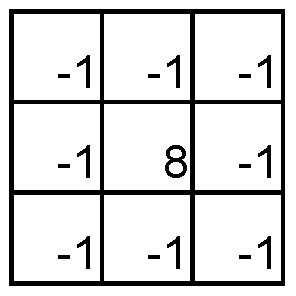
\includegraphics[width=3cm]{laplacian.pdf}
\end{center}
\caption{Operator Laplace'a}
\label{fig:laplacian_kernel}
\end{figure}

\begin{equation}
\label{eq:blobRadius}
r = \sigma \cdot \sqrt{2}
\end{equation}
gdzie:

$ \sigma $ - wariancja (parametr skali) wyznaczony podczas tworzenia filtru Gaussa dla danej skali.

\subsubsection{Rozpoznawanie krawędzi}
\label{subsubsec:rozpoznawanieKrawedzi}

Warunki istnienia krawędzi w~danym punkcie obrazu dla sygnału ciągłego są określone na równaniu \ref{eq:edgeDetection}.

\begin{equation}
\label{eq:edgeDetection}
\left\{ \begin{array}{rl}
L_x^2 L_{xx} + 2L_xL_yL_{xy} + L_y^2L_{yy} = 0 \\
L_x^3L_{xxx} + 3L_x^2L_yL_{xxy} + 3L_xL_y^2L_{xyy} + L_y^3L_{yyy} < 0
\end{array} \right.
\end{equation}

W~celu znalezienia krawędzi na obrazie, dla każdej skali wyznaczane są obrazy odpowiadające warunkom \ref{eq:edgeDetection}. Następnie każdy punkt obrazów reprezentacji skali jest sprawdzany czy warunki \ref{eq:edgeDetection} są spełnione. Jeśli tak to dany punkt jest uznawany za fragment krawędzi.

W~przypadku sygnałów dyskretnych problemem staje się miejsce występowania miejsc, w którym pierwszy warunek z \ref{eq:edgeDetection} jest spełniony. Nie jest to w punktach gdzie znajdują się piksele, lecz pomiędzy nimi. Z~tego powodu zmiast porównywania do zera w~warunku pierwszy sprawdzane jest czy zmienia się znak pomiędzy dwoma pikselami. Dla analizowanego piksela sprawdzany są jedynie trzy sąsiednie piksle oznaczone na rys. \ref{fig:comparePixels}. 


\subsubsection{Rozpoznawanie grani}
\label{subsubsec:rozpoznawanieGrani}

Warunk istnienia grani w~danym punkcie obrazu dla sygnału ciągłego są określone na równaniu \ref{eq:ridgeDetection}.



\subsubsection{Rozpoznawanie narożników}
\label{subsubsec:rozpoznawanieNaroznikow}


\section{Standard OpenCL}
\label{sec:OpenCL}

Ponieważ realizacja algorytmu Scale Space wymaga przeprowadzenia bardzo dużej liczby obliczeń, zdecydowano, że algorytm będzie zrealizowany z użyciem karty graficznej.

Do wykorzystania kart graficznych w~obliczeniach ogólnego przeznaczenia można zastosować otwarty standard OpenCL lub środowiska stworzone przez producentów procesorów graficznych dedykowanych dla urządzeń danego producenta.

OpenCL jest to otwarty, wieloplatformowy standard pozwalający na realizację algorytmów w~sposób równoległy. Umożliwia realizację jednego algorytmu (z~dokładnością do wspieranej wersji standardu) na wielu różnego typu ~urządzeniach. Wśród nich znajdują się procesory oraz karty graficzne dla komputerów osobistych działających
 pod kontrolą jednego popularnych systemów operacyjnych (Windows, Linux, OS X), telefony komórkowe, procesory ARM (również wielordzeniowe). Producenci wspierający obecnie standard to Intel,
QUALCOMM,
ARM,
AMD,
Apple,
Vivante Corporation,
STMicroelectronics International NV,
IBM Corporation,
Imagination Technologies,
Creative Labs.
Dzięki temu zastosowanie standardu pozwala stworzyć oprogramowanie, które może być wykorzystane w~praktycznie dowolnej konfiguracji urządzeń przetwarzających dane. Prace nad standardem rozpoczęły się w~2008 roku. Jest to technologia wciąż rozwijająca się oraz zapewniająca wsteczną kompatybilność. Obecnie istnieją 3 wersje standardu i~dotychczas wsteczna kompatybilność jest zapewniona. Jest to istotne z~uwagi na to, że różne urządzenia mogą nie wspierać nowszych wersji standardu, zwłaszcza jeśli zostały wyprodukowane przez wydaniem wersji standardu.

Przykładem środowisk stworzonych przez producentów procesorów graficznych dedykowanych dla urządzeń danego producenta są: CUDA firmy NVIDIA oraz ATI Stream. Środowiska te są ograniczone tylko do produktów jednego producenta, co znacznie zmniejsza przenośność stworzonej aplikacji. Powstały w~2006 roku. Znacznie bardziej znaną obecnie jest środowisko CUDA. Przedstawione alternatywy do OpenCL również są w~fazie intensywnego rozwoju oraz oferują wsteczną kompatybilność, to znaczy napisany kod będzie działał tak samo na nowszych wersjach danego środowiska, jak na poprzednich. Nie sprawdzono jak bardzo dane środowiska są zgodne z~tym założeniem.

Porównując wydajność OpenCL z rozwiązaniami opracowanymi przez różnych producentów kart graficznych należy zauważyć, że implementacje standardu są w~większości opracowywane przez producentów sprzętu wraz ze~sterownikami. W~związku z tym różnica w~efektywności działania nie istnieje lub jest znikoma (w~zależności od użytych instrukcji)\cite{FromCudaToOpenCL}. Dlatego ten aspekt nie był brany pod uwagę podczas wyboru środowiska do programowania kart graficznych.

Biorąc pod uwagę powyższe cechy standardu OpenCL oraz środowisk dedykowanych przez producentów sprzętu zdecydowano się na realizację algorytmu za pomocą OpenCL. Dzięki temu implementacja będzie mogła być wykorzystana w~różnych konfiguracjach sprzętowych.

